The ECal uses an adapted version of the clustering algorithm that was used by the CLAS IC. The geometrical arrangement of the crystals differs greatly from that used by the IC and required detailed studies and simulations to reconstruct the incident particle energy. The angles of incidence of the particles (electrons, positrons, and photons) entering the Ecal varies significantly across the ECal. The edge effects in the ECal are substantial due to the horizontal split between the top and bottom halves and  the proximity to the beam. \\
\indent Simulations were performed using the fully modeled detector geometry in SLIC as part of the standard hps software package. The geometry includes all strips of the SVT, vacuum chambers, ECal crystals, and relevant dead material. The geometry also moves particles through a 3D magnetic field map corresponding to the field values for 1~GeV beam running.~\cite{szumila-vance_hps_2016} \\
\indent Single particles: electrons, positrons, and photons were simulated at discrete energies of 0.2, 0.3, 0.4, 0.5, 0.6, 0.7, 0.8,  0.9, 1.0, and 1.1~GeV to uniformly cover the ranger of energies detectable in the Engineering Run. The simulation uses the full reconstruction chain excluding pile-up effects. The offline cluster reconstruction uses the same thresholds used in data and production Monte Carlo: 7.5~MeV for individual hits, 50~MeV for seed hits in clusters, and 100~MeV for cluster energies.\\

\subsubsection{Energy reconstruction}
\indent Due to the complex showering cascade that occurs when a particle deposits its energy in the ECal, several adjacent crystal modules contain some fraction of the incident energy of the particle. These modules are clustered in offline reconstruction to obtain the total deposited energy of the incident particle. The reconstructed energy not corrected for shower loss effects is defined by Equation~\eqref{eq:eclsum}.

\begin{equation}
\label{eq:eclsum}
E_{rec} = \sum_i E_i    
\end{equation}

In Equation~\eqref{eq:eclsum}, the subscript $i$ pertains to each module in the cluster such that $E_i$ is the energy of each module in the cluster. Some incident particle energy is lost between crystals and out the back where the APD does not fully cover the surface of each crystal. After recovering the energy as measured by the ECal, the incident particle energy can be found by correcting for the shower loss effects as described by Equation~\eqref{eq:eclsf}.

\begin{equation}
\label{eq:eclsf}
E_{corr} = \dfrac{E_{rec}}{f}   
\end{equation}

In Equation~\eqref{eq:eclsf}, $f$ is the energy-dependent ratio of measured vs incident particle energy. This factor is obtained through simulation. The energy loss corrections as derived from Monte Carlo are shown in Fig.~\ref{Figure:ecorr} where $E_{gen}$ refers to the simulated Monte Carlo particle energy.

\begin{figure}[thb]
  \centering
      \includegraphics[width=0.75\textwidth]{pics/performance/energycorrection.pdf}
  \caption[ECal energy shower correction functions from simulation]{Energy correction functions correct the energy measured in the ECal to reconstruct the energy of the incident particle.}
  \label{Figure:ecorr}
\end{figure}

The difference in the energy corrections for the various particle types arises from geometrical effects and the incident angles of the particles entering the crystals.~\cite{szumila-vance_hps_ecal_2014} The focal point of the calorimeter, the point at which all crystals are angles, lies 80~cm from the front face of the ECal. The HPS target is beyond this focal distance at approximately 1.3~m from the face of the ECal and is offset beam right in the pair spectrometer magnetic field. Particles produced at the target take different trajectories from the target to the ECal due to the interactions of their charge and momentum in the magnetic field. This affects the entry angle of the particle into a crystal and mandates a charge and momentum-dependent energy correction function. The form of the energy correction function for the central region of the ECal is described by a three parameter fit in Eq.~\eqref{eq:ecorrfunc}.

\begin{equation}
	\label{eq:ecorrfunc}
	\dfrac{E_{rec}}{E_{gen}} = \dfrac{A}{E_{rec}}+\dfrac{B}{\sqrt{E_{rec}}}+C 
\end{equation}

The shower leakage effects in crystals becomes significant at distances close to the edge. The energy reconstruction deteriorates rapidly in the crystals closest to the edge but stabilizes in central region of the ECal. The energy reconstruction at the edges was fully characterized using Monte Carlo as a function of position in the ECal relative to the inner beam gap edge. In Equation ~\eqref{eq:ecorrfunc}, parameter $A$ is not strongly correlated with position and remains as a constant for a given particle type. The parameters $B$ and $C$  do depend on cluster position relative to the beam gap edge of the ECal. These dependencies can be seen for electrons in Fig.~\ref{Figure:sfparEdge}.

\begin{figure}[H]
  \centering
      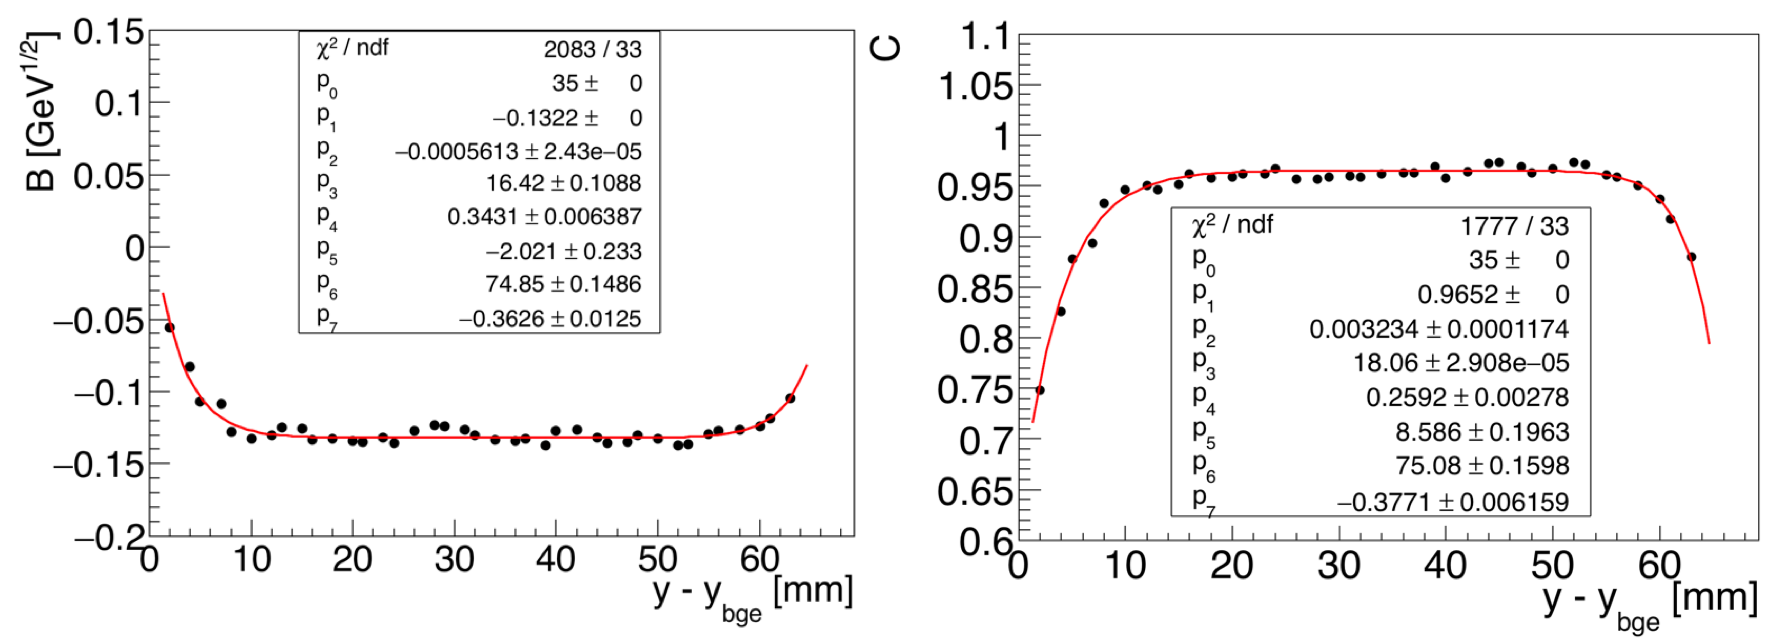
\includegraphics[width=1.0\textwidth]{pics/performance/sfparEdgeFit.png}
  \caption[ECal energy shower parameters for electrons relative to the inside beam gap edge]{Parameters $B$ and $C$ from Eq.~\ref{eq:ecorrfunc} for electrons, as a function of vertical position
relative to the innermost beam gap edge.}
  \label{Figure:sfparEdge}
\end{figure}

As shown in Fig.~\ref{Figure:sfparEdge}, the energy leakage parameters $B$ and $C$ can be fit with two functions at the edges that match in the central region of the ECal, away from the edges of the calorimeter. The equations used to fit the $B$ and $C$ parameters are described by Equations ~\eqref{eq:p1parlt} and ~\eqref{eq:p2parlt}, respectively.

\begin{equation}
\begin{split}
\label{eq:p1parlt}
B(y<p_0) = p_1-p_2 e^{-(y-p_3)p_4}\\
B(y>p_0) = p_1-p_5 e^{-(y-p_6)p_7}
\end{split}
\end{equation}

\begin{equation}
\begin{split}
\label{eq:p2parlt}
C(y<p_0) = p_1-p_2 e^{-(y-p_3)p_4}\\
C(y>p_0) = p_1-p_5 e^{-(y-p_6)p_7}
\end{split}
\end{equation}

The energy leakage correction functions are relatively constant in the central region of the calorimeter and are matched at a central distance $p_0$. For columns containing 5 crystals vertically, the distance to the beam gap edge is the absolute value of the distance from the cluster centroid to the innermost beam gap edge. In the regions above and below the region where row 1 crystals are removed in the ECal, additional consideration is made when calculating the distance to the inner beam gap edge in order to be consistent with other regions of the ECal. For completeness, the corresponding energy correction parameters for positrons and photons are seen in Figures~\ref{Figure:sfparEdgeEP} and \ref{Figure:sfparEdgeP}, respectively. 


\begin{figure}[H]
  \centering
      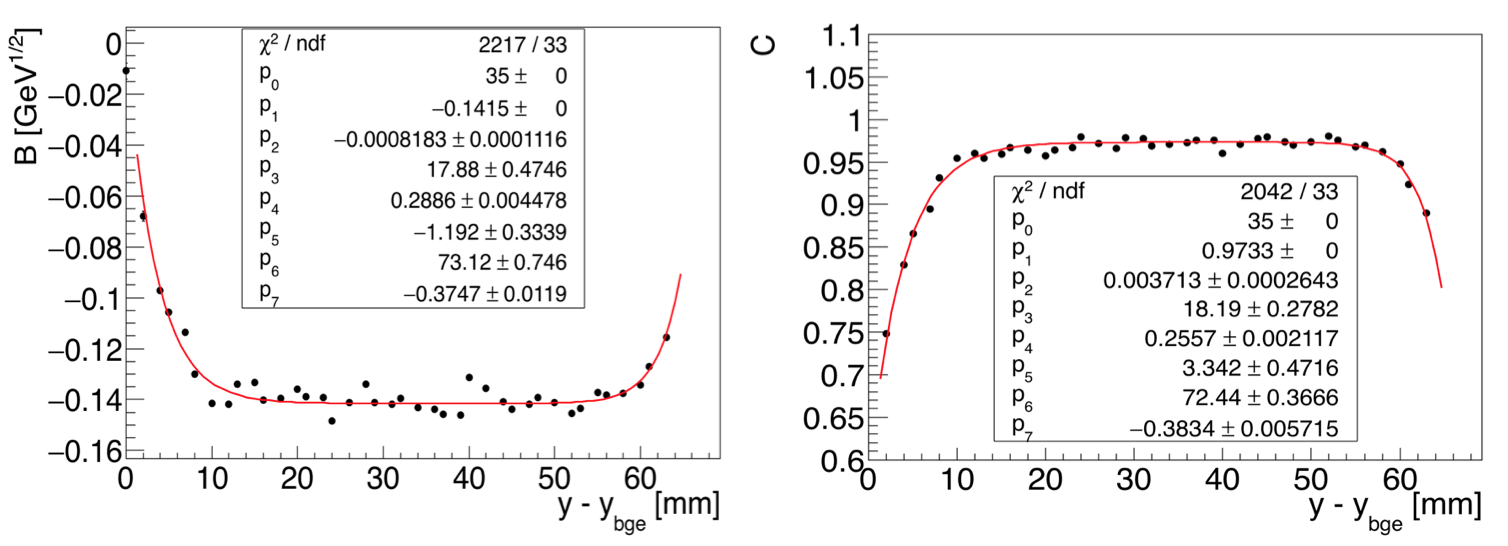
\includegraphics[width=1.0\textwidth]{pics/performance/sfparEdge_ep.png}
  \caption[ECal energy shower parameters for positrons relative to the inside beam gap edge]{Parameters $B$ and $C$ from Eq.~\ref{eq:ecorrfunc} for positrons, as a function of vertical position
relative to the innermost beam gap edge.}
  \label{Figure:sfparEdgeEP}
\end{figure}

\begin{figure}[H]
  \centering
      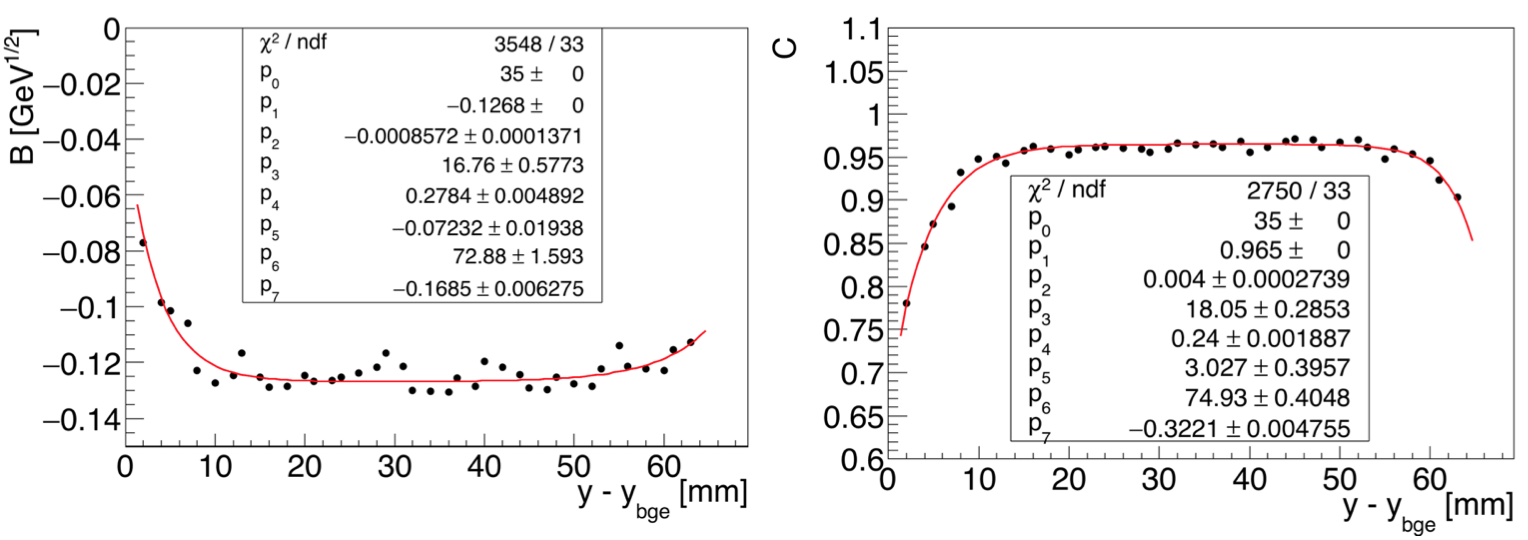
\includegraphics[width=1.0\textwidth]{pics/performance/sfparEdge_p.png}
  \caption[ECal energy shower parameters for photons relative to the inside beam gap edge]{Parameters $B$ and $C$ from Eq.~\ref{eq:ecorrfunc} for photons, as a function of vertical position
relative to the innermost beam gap edge.}
  \label{Figure:sfparEdgeP}
\end{figure}

As one can see, the energy corrections are relatively constant at approximately 1~cm from the edges of the ECal. As a result, we define the fiducial the region of the ECal to be at greater than 1~cm from the edge, or approximately 3/4 of the font face crystal dimension. This result is consistent with the findings for the CLAS IC.~\cite{szumila-vance_hps_ecal_2014} 

\subsubsection{Energy resolution}

The energy resolution of the ECal is energy-dependent and improves with energy as $1/\sqrt{E}$. From simulation, we obtain the energy resolution as shown in Figure~\ref{Figure:eResFitMC}.

\begin{figure}[H]
  \centering
      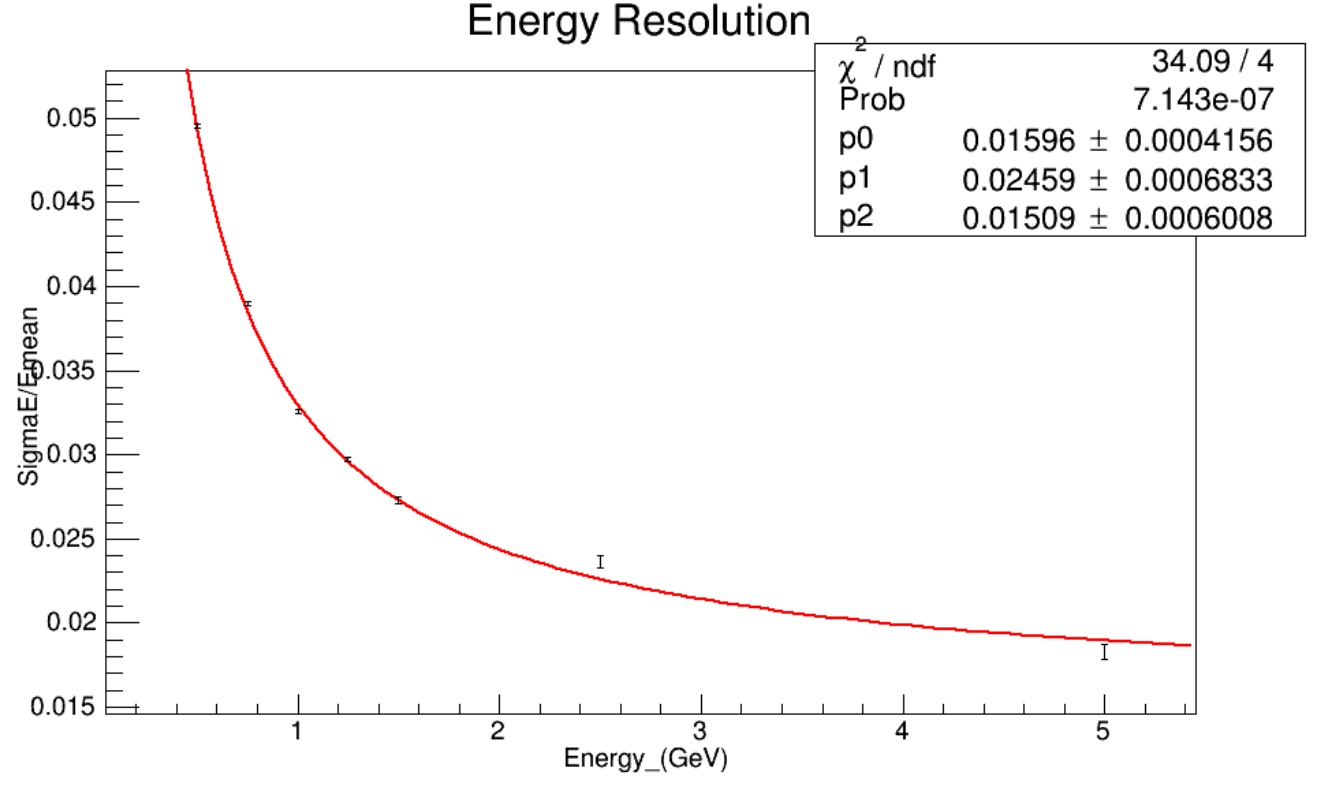
\includegraphics[width=0.6\textwidth]{pics/performance/eResFitMC.png}
  \caption[ECal energy resolution fitted from simulation]{ECal energy resolution from simulation.}
  \label{Figure:eResFitMC}
\end{figure}

The fit shown in Figure~\ref{Figure:eResFitMC} is described by Equation~\ref{eq:eResMC}.

\begin{equation}
\label{eq:eResMC}
\dfrac{\sigma_E}{E} (\%) = \dfrac{1.60}{E} \oplus \dfrac{2.46}{\sqrt{E}} \oplus 1.51
\end{equation}

The first term corresponds to the preamplifier noise. We were expecting 3~MeV$\times \sqrt{10} = 0.009$~GeV, where 10 is the average number of hit crystals. This term from simulation is not including the FADC error (expected to be 1.3~MeV~\cite{charles_2014}) which contributes a term (in $\%$) as $0.13\sqrt{10}/E$ to be added, quadratically. The second term corresponds to the statistical fluctuations in the shower development and is influenced by the lateral containment of the shower and energy deposited in the crystal module. The second term from simulation is not including fluctuations in the number of photoelectrons (30 photoelectrons/MeV, multiplied by an excess noise factor parameterizing the fluctuations in the APD gain process, or Fano factor, of 2~\cite{panda_2008}) contributing $0.8/\sqrt{E}$. This term is calculated as $\sqrt{F/N_{pe/GeV}}$. The third term is interpreted as the fluctuation of energy leakage through the back of the crystals. This third term should includ the crystal-to crystal inter-calibration error which estimate to be 1~$\%$.~\cite{szumila-vance_hps_ecal_2014} By including these additional resolution effects in the measurement, we obtain the resolution as anticipated from Monte Carlo in Equation~\eqref{eq:eResUpdated}.

\begin{equation}
\label{eq:eResUpdated}
\dfrac{\sigma_E}{E} (\%) = \dfrac{1.65}{E} \oplus \dfrac{2.59}{\sqrt{E}} \oplus 1.81 
\end{equation}

\subsubsection{Position reconstruction}
\indent ECal clusters provide position information of comparable resolution to the SVT. Various weighting schemes for calculating a cluster centroid can be problematic due to periodic patterns resulting from the segmentation of the crystals. The same weighting scheme, used by the CLAS IC algorithm, provided the optimal position resolution. The calculation of the position of the cluster is shown in Equation~\eqref{eq:posncalc}.~\cite{szumila-vance_hps_ecal_2014}

\begin{eqnarray*}
\label{eq:posncalc}
x_{cl} & = & \dfrac{\sum_i w_i x_i}{\sum_i w_i}\\
y_{cl} & = & \dfrac{\sum_i w_i y_i}{\sum_i w_i}\\
\end{eqnarray*}

In Equation~\eqref{eq:posnwt}, the index $i$ indicates the individual module in the cluster, and $w_i$ is described by Equation~\eqref{eq:posnwt}.

\begin{equation}
\label{eq:posnwt}
w_i  =  max[0, w_0+ ln\dfrac{E_i}{E_{rec}}]
\end{equation}

The parameter $w_0$ in Equation~\eqref{eq:posnwt} is an energy threshold such that $E_i/E_{cl} > e^{-w_0}$ and is found in simulation to have a value of $3.1$ \cite{szumila-vance_hps_ecal_2014}. The logarithmic term enhances the contribution from the tails and improves the position measurement. Additional effects resulting from the differing angles of entry at the ECal require a position correction to the $x$-coordinate of the cluster. These corrections are both charge and momentum-dependent. The position correction for a generated 1~GeV electron is shown in Figure~\ref{Figure:xposn1gev}.

\begin{figure}[H]
  \centering
      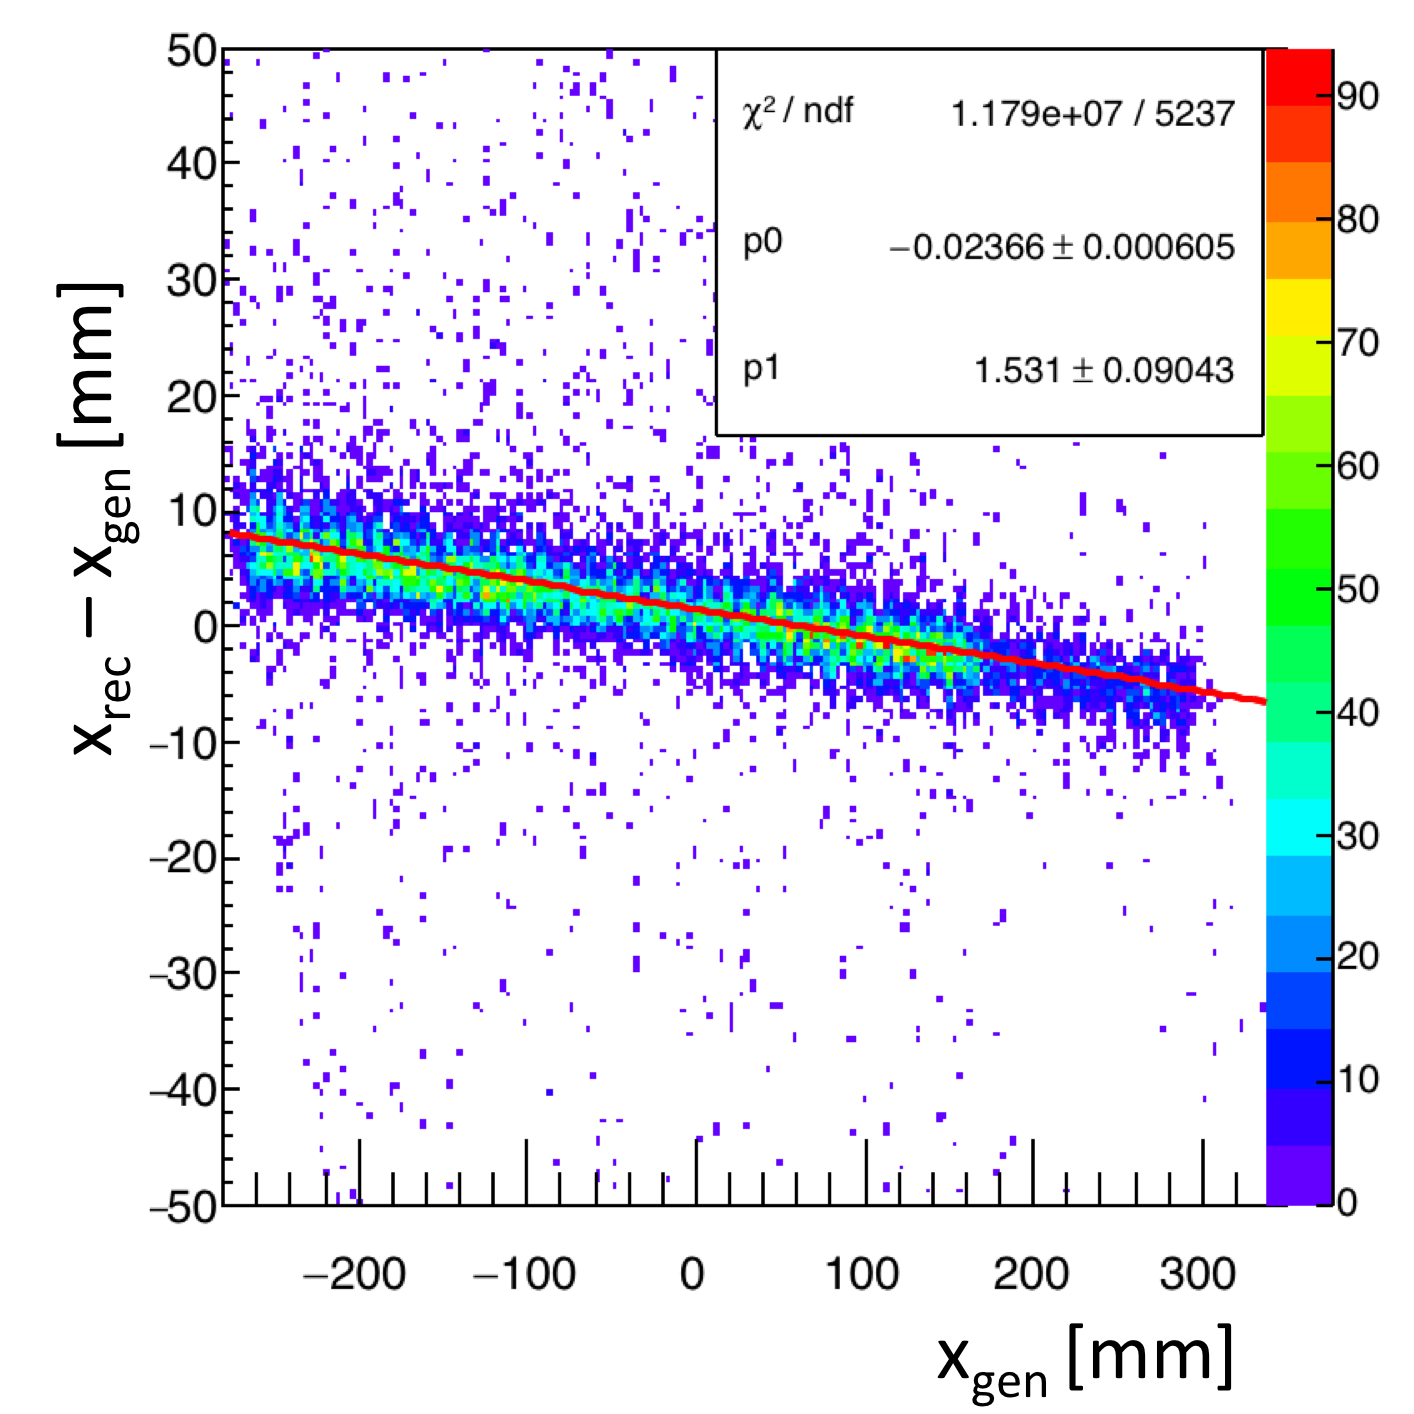
\includegraphics[width=0.7\textwidth]{pics/performance/xposn1gev.png}
  \caption[Horizontal position correction for 1~GeV electrons]{The position correction as found for a 1~GeV electron is both energy and position-dependent in order to account for the different angle of incidence at the ECal.}
  \label{Figure:xposn1gev}
\end{figure}

The correction at each energy by particle-type is fit with Equation~\eqref{eq:posncorr}. 

\begin{equation}
\label{eq:posncorr}
x_{rec} - x_{gen} = A(E_{rec}) x_{gen} + B(E_{rec})
\end{equation}

The energy-dependence of the fit parameters $A(E_{rec})$ and $B(E_{rec})$ use the reconstructed cluster energy, uncorrected for shower loss effects. These parameters for the electron horizontal position correction as a function of the reconstructed cluster energy are shown Figure~\ref{Figure:xposcorrPar}.

\begin{figure}[H]
  \centering
      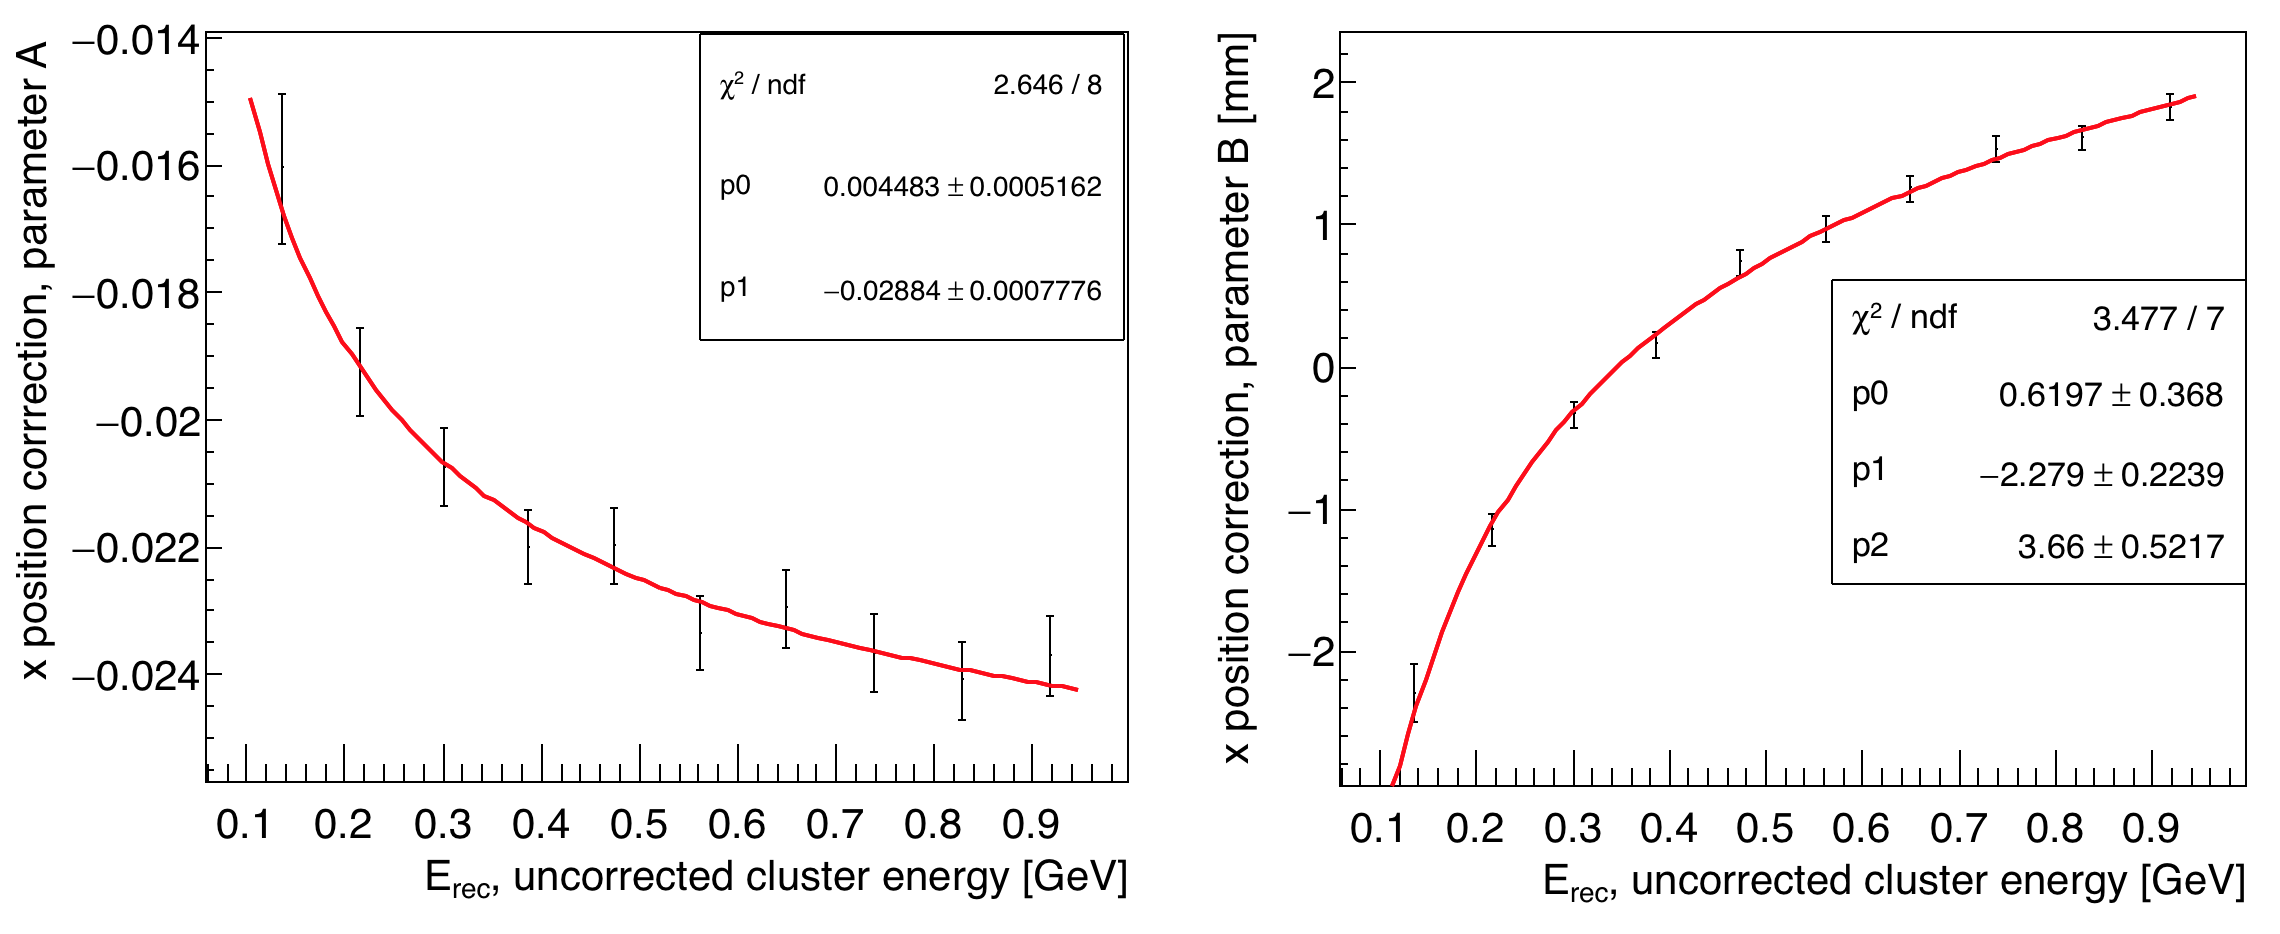
\includegraphics[width=1.0\textwidth]{pics/performance/xposcorrPar.png}
  \caption[Horizontal position correction dependence for electrons]{The horizontal position correction parameters as functions of the uncorrected cluster energy.}
  \label{Figure:xposcorrPar}
\end{figure}

The parameters in Figure~\ref{Figure:xposcorrPar} are fit to functions of the form described in Equation~\eqref{eq:posnCpar}.

\begin{eqnarray*}
\label{eq:posnCpar}
A(E_{rec}) & = & \dfrac{p0}{\sqrt{E_{rec}}}+p1\\
B(E_{rec}) & = & p0\times E_{rec} +\dfrac{p1}{\sqrt{E_{rec}}}+p2
\end{eqnarray*}

The corresponding correction values for all three particle types can be summarized in Table~\ref{tab:horizPosCorr}.

\begin{table}[H]
\caption{Horizontal position corrections.}
\label{tab:horizPosCorr}
\centering
\begin{tabular}{|c|c|c|}
\toprule
%\multicolumn{2}{c}{Name} \\
%\cmidrule(r){1-2}
Particle & $A(E_{rec})$ & $B(E_{rec})$ \\
\midrule
electron & $0.004483/\sqrt{E_{rec}}-0.02884$ & $0.6197E_{rec}-2.279/\sqrt{E_{rec}}+3.66$ \\
positron & $0.006887/\sqrt{E_{rec}}-0.03207$ & $-0.8048E_{rec}+0.9366/\sqrt{E_{rec}}+2.628$ \\
photon & $0.005385/\sqrt{E_{rec}}-0.03562$ & $-0.1948E_{rec}-0.7991/\sqrt{E_{rec}}+3.797$ \\
\bottomrule
\end{tabular}
\end{table}

Position corrections are not needed for the vertical cluster position.

\subsubsection{Position resolution}

After applying the position corrections to each particle-type at the simulated energies, the residual between the measured and simulated position reconstruction is obtained is measured. The fitted residuals after correcting the position of 1~GeV electron clusters are shown in Figure~\ref{Figure:corrPosnsFits}.

\begin{figure}[H]
  \centering
      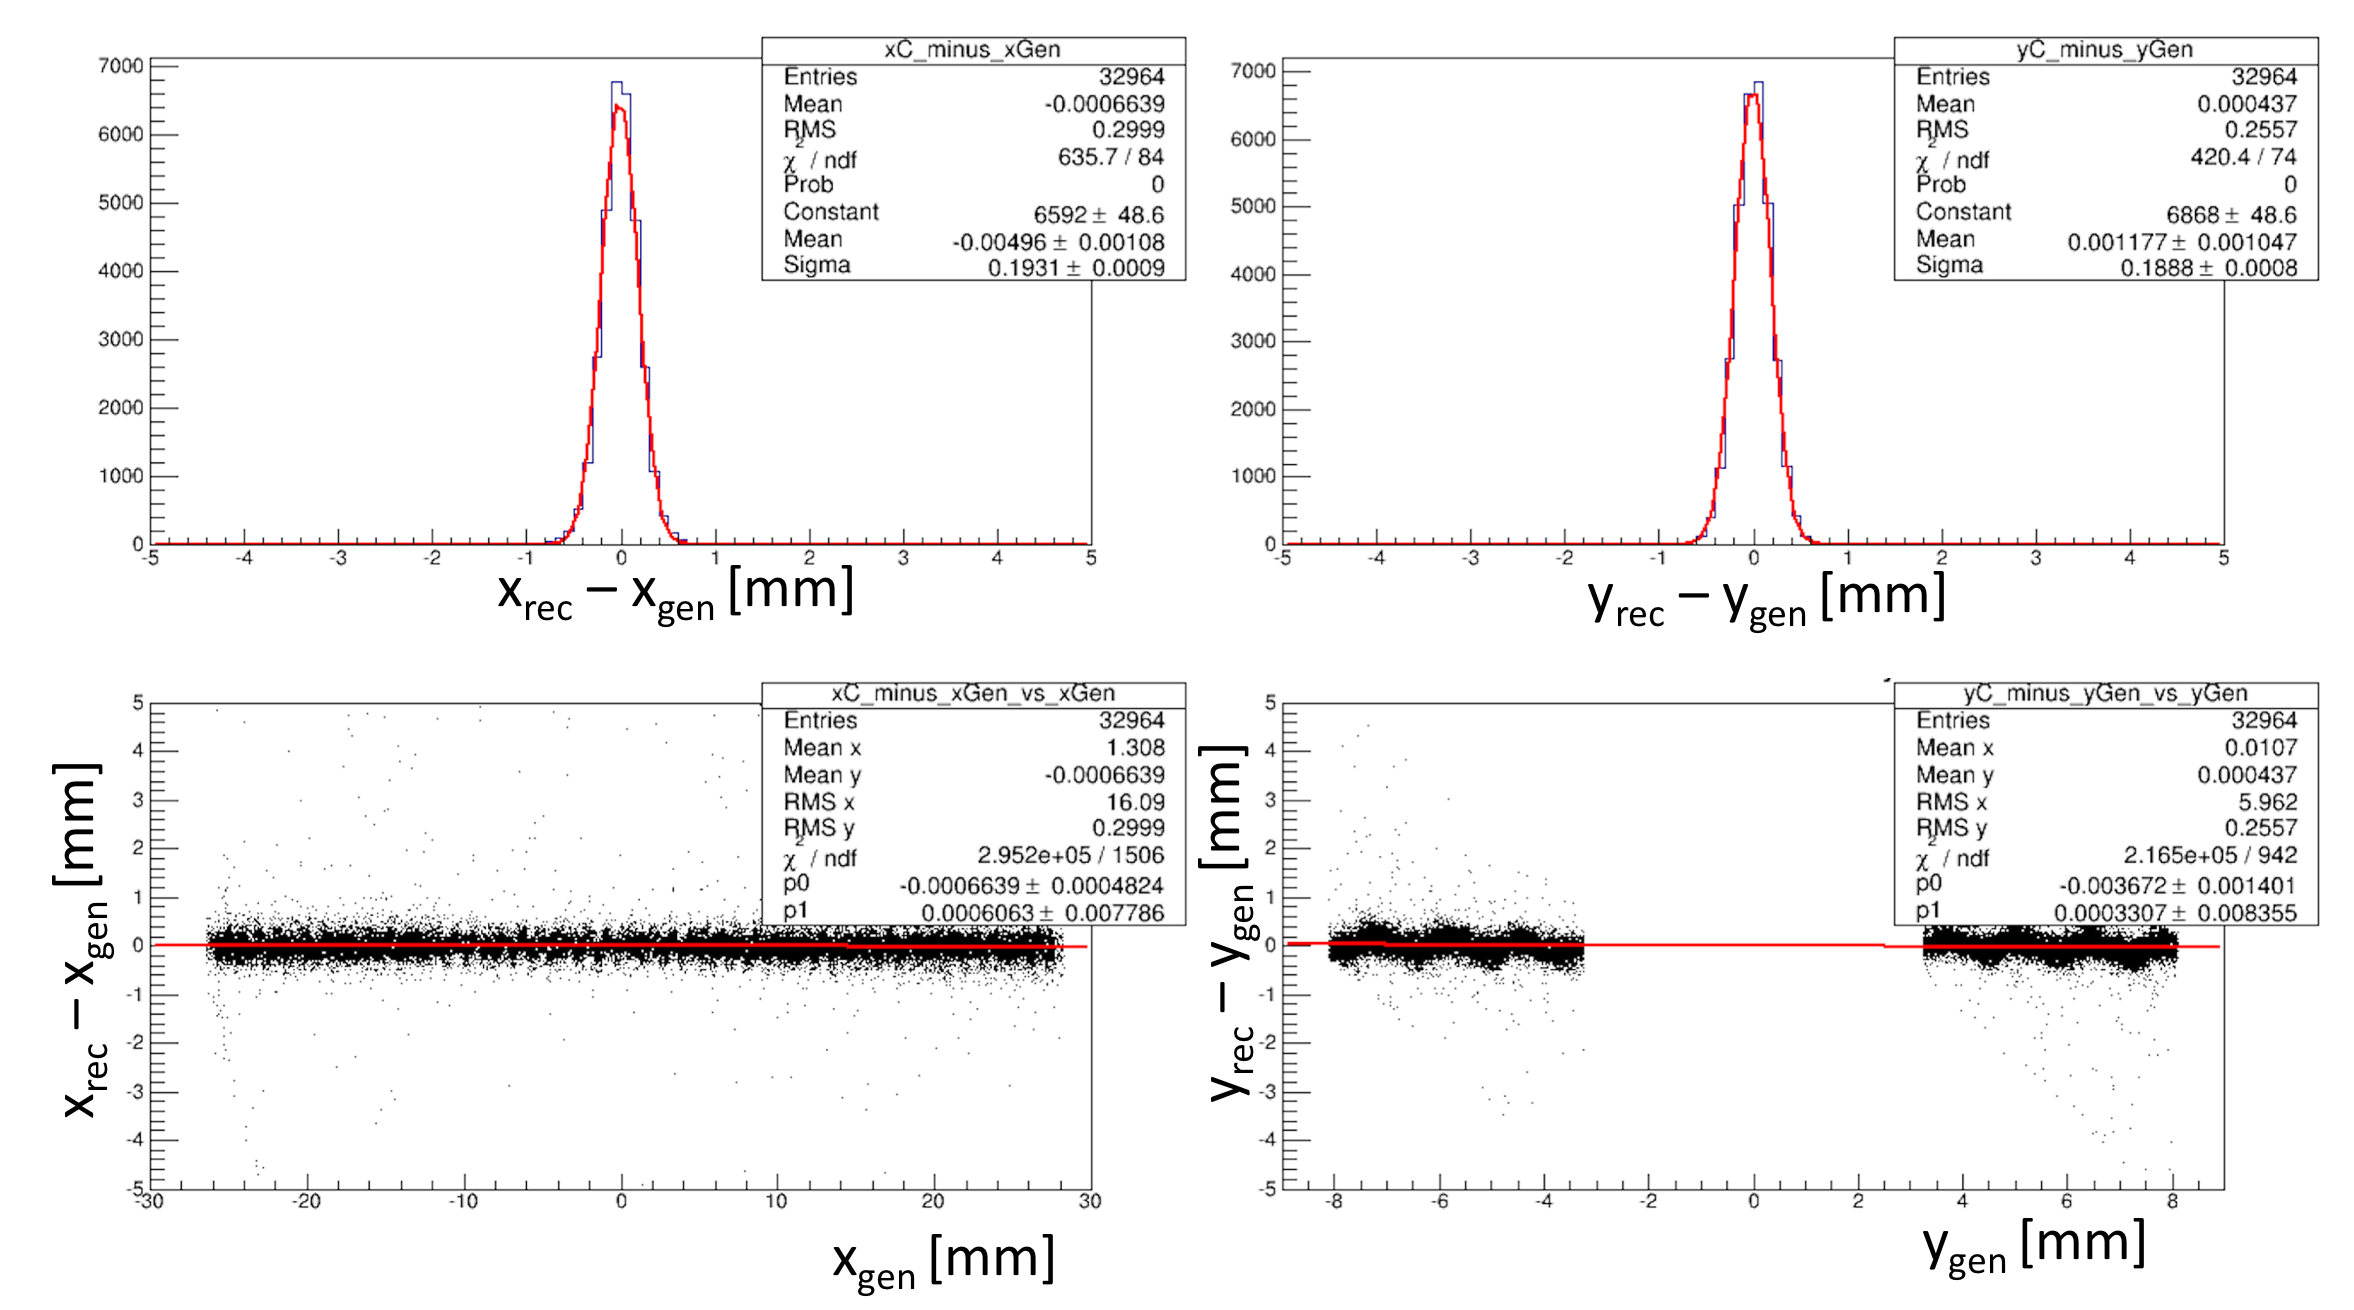
\includegraphics[width=1.0\textwidth]{pics/performance/corrPosnsFits.png}
  \caption[Position resolution for 1~GeV electrons.]{The position resolution for 1~GeV electrons, after applying the horizontal position corrections.}
  \label{Figure:corrPosnsFits}
\end{figure}

As shown in Figure~\ref{Figure:corrPosnsFits}, no correction is required when reconstructing the vertical position of the cluster. The energy-dependent resolution of both the horizontal and vertical position of reconstructed clusters can be seen for electrons in Figure~\ref{Figure:emPosnResn}. 

\begin{figure}[H]
  \centering
      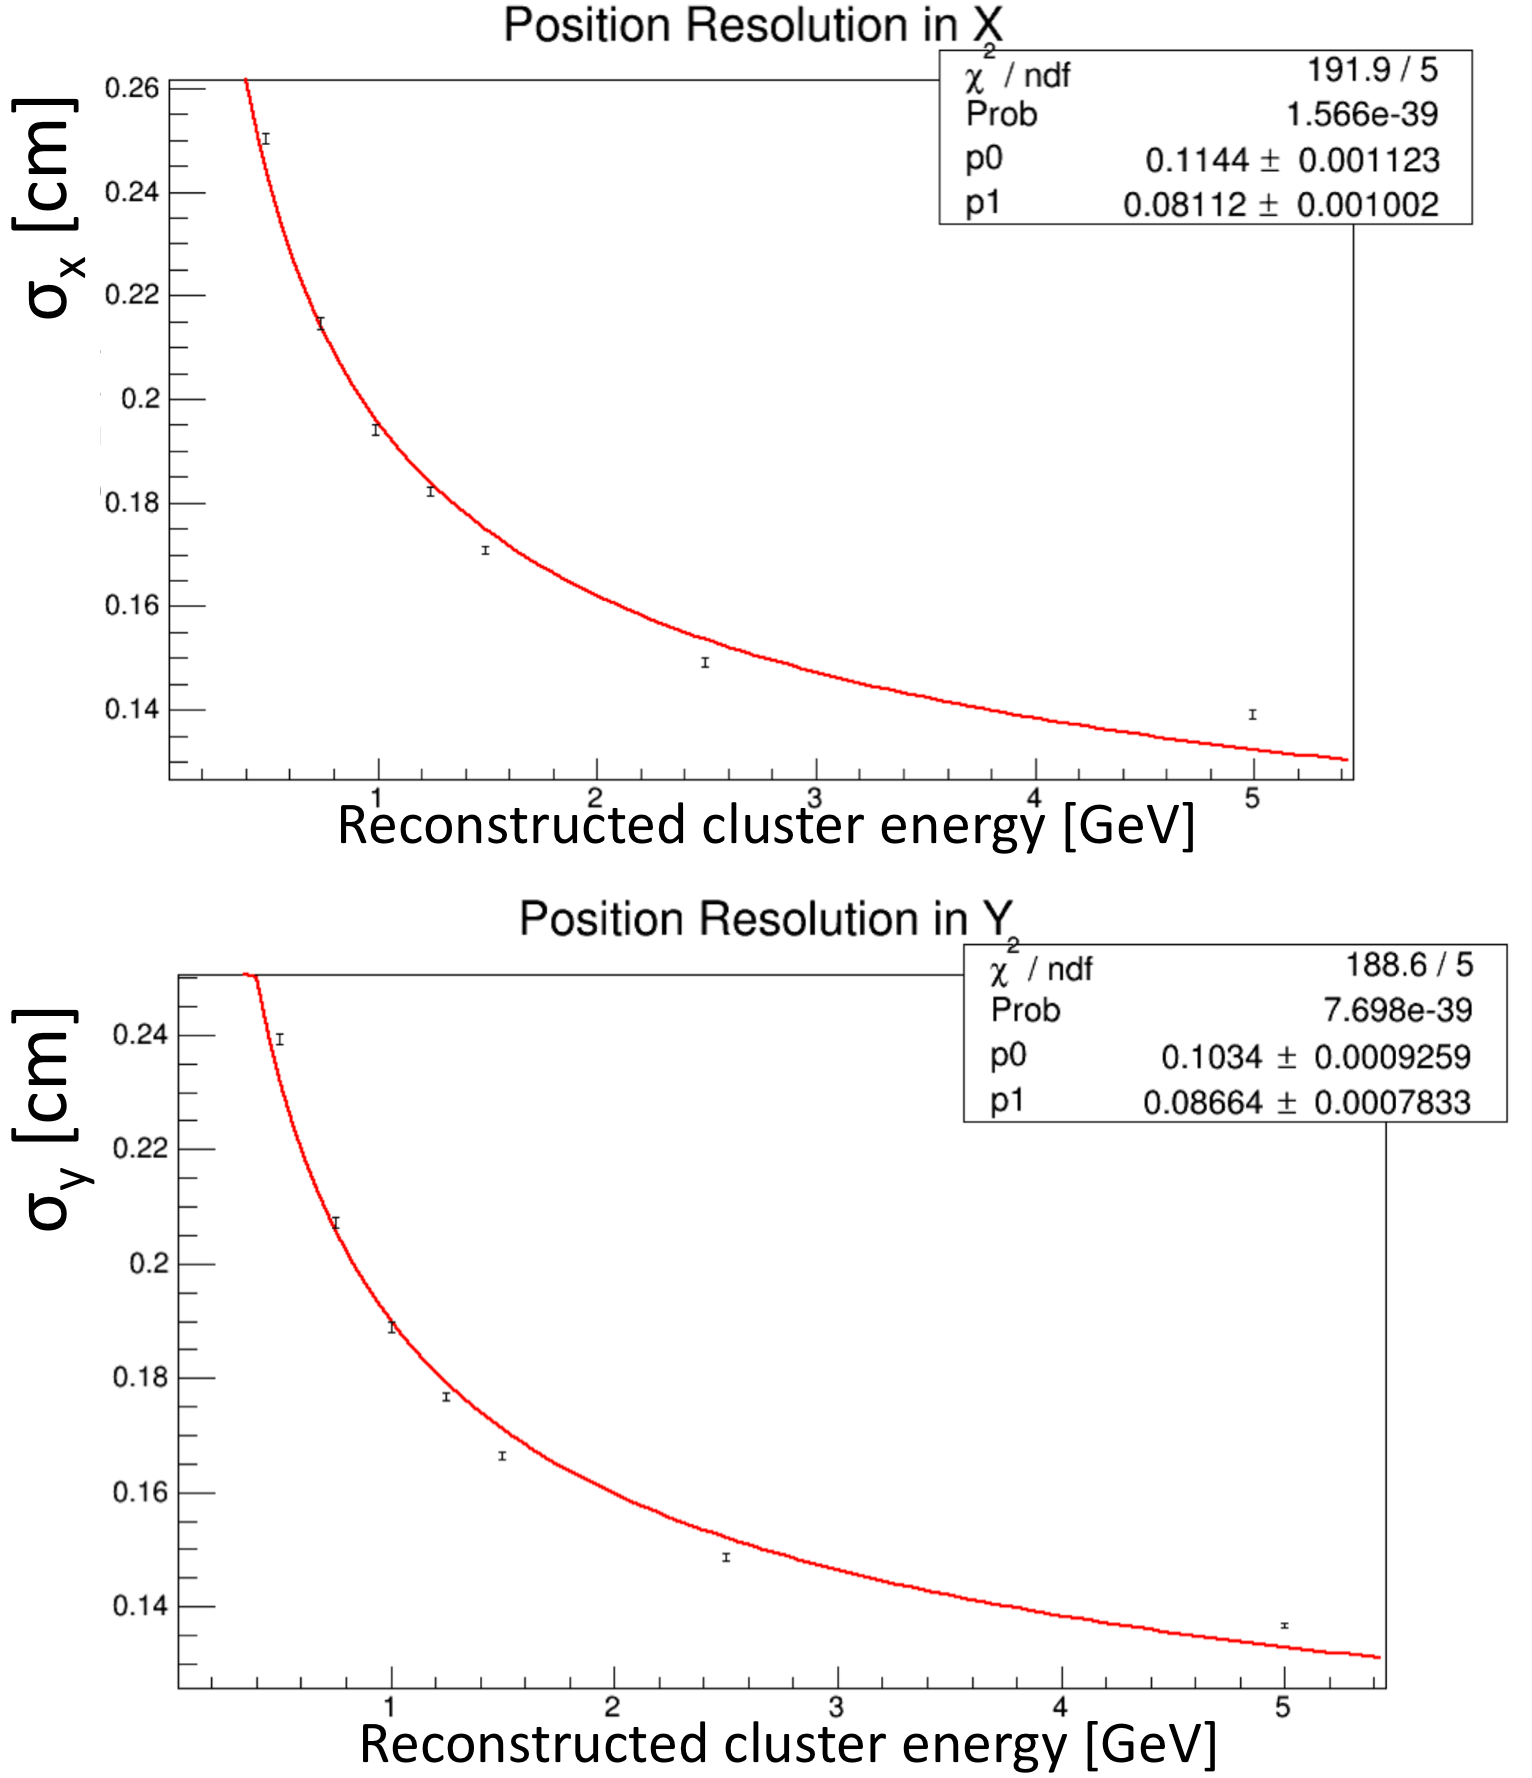
\includegraphics[width=0.9\textwidth]{pics/performance/emPosnResn.png}
  \caption[Energy-dependent position resolution for electrons.]{The energy-dependence of the position resolution for electrons.}
  \label{Figure:emPosnResn}
\end{figure}

The position resolution is parameterized in terms energy following Equation~\eqref{eq:posnRes}.
 
\begin{eqnarray*}
\label{eq:posnRes}
\sigma_x & = & \dfrac{p0_x}{\sqrt{E}}+p1_x\\
\sigma_y & = & \dfrac{p0_y}{\sqrt{E}}+p1_y
\end{eqnarray*}

The parameters $p0$ and $p1$ are found by fitting the residuals for the energies. The position resolution is better than 2~mm for 1~GeV electrons. As the ECal face is located at  approximately 1.4~m from the target, the ECal provides valuable position information when matched with a track. The position resolution for all particle types in the ECal is summarized in Table~\ref{tab:PosnResTable}. 

\begin{table}[H]
\caption{Position resolution.}
\label{tab:PosnResTable}
\centering
\begin{tabular}{|c|c|c|}
\toprule
%\multicolumn{2}{c}{Name} \\
%\cmidrule(r){1-2}
Particle & $\sigma_x$ [mm] & $\sigma_y$ [mm] \\
\midrule
electron & $0.1144/\sqrt{E_{rec}}+0.08112$ & $0.1034/\sqrt{E_{rec}}+0.08664$ \\
positron & $0.1268/\sqrt{E_{rec}}+0.07711$ & $0.1068/\sqrt{E_{rec}}+0.08423$ \\
photon & $0.1255/\sqrt{E_{rec}}+0.08877$ & $0.1005/\sqrt{E_{rec}}+0.08867$ \\
\bottomrule
\end{tabular}
\end{table}